%% Copyright (C) 2013 by Armando Fox.  All rights reserved.

\documentclass{article}

\usepackage{times}

\usepackage{ifthen}
\usepackage{xstring} % needed by wikipedia macro
\usepackage{fullpage}
\usepackage{hyperref}
\usepackage{fancybox}
%\usepackage[square,comma,authoryear]{natbib}
\usepackage{graphicx}

\usepackage[T1]{fontenc}

\title{In Praise of BASIC: The Cultural Impact of the World's Most
  Maligned Programming Language}
\author{Armando Fox}

\begin{document}
\newif\ifhtmloutput\htmloutputfalse
\newif\ifmobioutput\mobioutputfalse

\newcommand{\T}{\texttt}
\newcommand{\B}{\textbf}
\newcommand{\Sf}[1]{\textsf{\emph{#1}}}
\newcommand{\C}[1]{\textsf{\upshape{\textbf{#1}}}}

%% "Geeknote" icon: footnotes/sidebars of interest primarily to geeks.  Can
%% be turned on/off in HTML/ebook version

\newcommand\geeknote\footnote  % for now


% Sidebar - appearance will vary depending on output target, and may not
% actually be along the side.
% Example use:
%   \begin{sidebar}{Historical note}
%     All this stuff will be in a sidebar.
%     You can include most elements that would go in normal text, like
%     figures, citations, etc.
%   \end{sidebar}
\setlength\fboxsep{2pt}

\newcommand{\sidebarfont}{%
  \fontencoding{\encodingdefault}%
  \fontfamily{phv}%
  \fontseries{mc}%
  \fontshape{\shapedefault}%
  \footnotesize
  \selectfont}


\definecolor{SidebarColor}{rgb}{0.9,0.9,0.9}
\ifhtmloutput
  \newenvironment{sidebar}[2][]%
    {\HCode{<span class="sidebar_name"><b><i>}#2{\HCode{</i></b></span>}}}
    {}
\else
  \newcommand{\thesidebarraise}{}
  \newenvironment{sidebar}[2][-2ex]%
    {\renewcommand{\thesidebarraise}{#1}%
     \begin{Sbox}\begin{minipage}{\marginparwidth}\sidebarfont\raggedright \textbf{#2}}%
    {\end{minipage}\end{Sbox}\marginpar{\vspace{\thesidebarraise}\colorbox{SidebarColor}{\TheSbox}}}
\fi

% Sidebars with photos - need to be small in PDF Output
% Small Kindle is 520x622 px; images 260x311 or smaller won't be resized on device
\ifmobioutput
    \newenvironment{sidebargraphic}[3][]%
      {\HCode{<img class="person" width="150" src="#2_SB.jpg"/>}
       \HCode{<span class="sidebar_name"><b><i>}#3{\HCode{</i></b></span>}}}
      {}
\else
  \newcommand{\thesidebarimg}{}% hack- numbered params can't appear in end content of \newenvironment
  \newenvironment{sidebargraphic}[3][0in]%
    {\renewcommand{\thesidebarraise}{#1}%
     \renewcommand{\thesidebarimg}{#2}%
     \begin{Sbox}\begin{minipage}{\marginparwidth}\sidebarfont\raggedright \textbf{#3}}%
    {\hfill\\ \vspace{0.75ex}\includegraphics[width=\marginparwidth]{\thesidebarimg}\end{minipage}\end{Sbox}\marginpar{\vspace{\thesidebarraise}\colorbox{SidebarColor}{\TheSbox}}}
\fi


% Quotation in small-ish type with attribution
% Example use:  
%  \makequotation{There's a sucker born every minute.}{W.C. Fields}

\ifhtmloutput
 \ifmobioutput
  \newcommand{\makequotation}[2]{\HCode{%
     <div class="makequotation" align="center">
      <table cellpadding="10" style="margin-left: 0;">
        <tr><td align="center" border="1" style="background-color: \#c0c0c0">}%
        #1\HCode{<i>} #2\HCode{</i>
        </td></tr>
      </table>
     </div>}}
 \else
  \newcommand{\makequotation}[2]{\begin{quote}\small\emph{#1} ---#2\end{quote}}
 \fi
\else
  \newcommand{\makequotation}[2]{\begin{quote}\small\emph{#1}

  \hfill---#2\end{quote}}
\fi


% Wikipedia link
%\usepackage{ifthen}
%\usepackage{xstring}  % provides StrSubstitute
\newcommand{\w}[2][]{%
  \ifhtmloutput
    \ifthenelse{\equal{#1}{}}{%
      \StrSubstitute{#2}{ }{_}[\thewikilink]%
      \weblink{http://en.wikipedia.org/wiki/\thewikilink}{\emph{\B{#2}}}%
    }{%
      \StrSubstitute{#1}{ }{_}[\thewikilink]%
      \weblink{http://en.wikipedia.org/wiki/\thewikilink}{\emph{\B{#2}}}%
    }%
  \else%
    \textsf{\slshape{#2}}%
  \fi%
  \ifhtmloutput%
  \else%
    \index{#2}%
    \ifthenelse{\equal{#1}{}}{}{\index{#1}}%
    \relax%
  \fi%
}

% online-glossary term
\newcommand{\x}[1]{\emph{\B{#1}}}

% ``REMark''
\setcounter{section}{9}
\newcommand{\mysection}[1]{%
  \section{REM~~{#1}} 
  \addtocounter{section}{9}
}

\newcommand{\smallpicfigure}[4][0.4]{
  \begin{wrapfigure}{R}{#1\textwidth}
    \centering
    \includegraphics[width=#1\textwidth]{#2}
    \caption{\label{#3}\textsf{#4}}
  \end{wrapfigure}}
\newcommand{\picfigure}[4][width=\textwidth]{%
  \begin{figure}
   \includegraphics[#1]{#2}
   \ifthenelse{\equal{#4}{}}{}{\caption{\label{#3}\textsf{#4}}}
  \end{figure}}

% table figures - will eventually do something different for mobi
\newcommand{\tablefigure}[3]{%
  \begin{figure}
    \small\input{#1}
    \caption{\label{#2}%
#3}
  \end{figure}
}

% Code - uses \verbatiminput to put in file 'undecorated' for HTML use,
% or \lstlisting to decorate it with styling and line numbers for PDF
\ifmobioutput
  \newcommand{\codefile}[2][]{\HCode{<a class="gist" href="https://gist.github.com/#1">https://gist.github.com/#1</a><br/><pre class="code">}

    \begin{minipage}{\textwidth}% prevent gratuitous blank lines
    \verbatiminput{#2}%
    \end{minipage}%
    \HCode{</pre><hr>}}
\else
  \newcommand{\codefile}[2][u/saasbook]{%
    \noindent\begin{minipage}{\textwidth}%
    \Sf{\scriptsize{}http://pastebin.com/#1}%
    \vspace{-1ex}%
    \lstinputlisting{#2}%
    \end{minipage}}
\fi


%  Code file 'figure'
\newcommand{\codefilefigure}[4][]{%  filename, reflabel, caption
  \begin{figure}
  \codefile[#1]{#2}
  \caption{\label{#3}
   \footnotesize #4
  }
  \end{figure}%
}



\maketitle


\makequotation{It is practically impossible to teach good programming to
  students that have had a prior exposure to BASIC: as potential
  programmers they are mentally mutilated beyond hope of
  regeneration.}{Edsger W. Dijkstra, Turing Award winner}

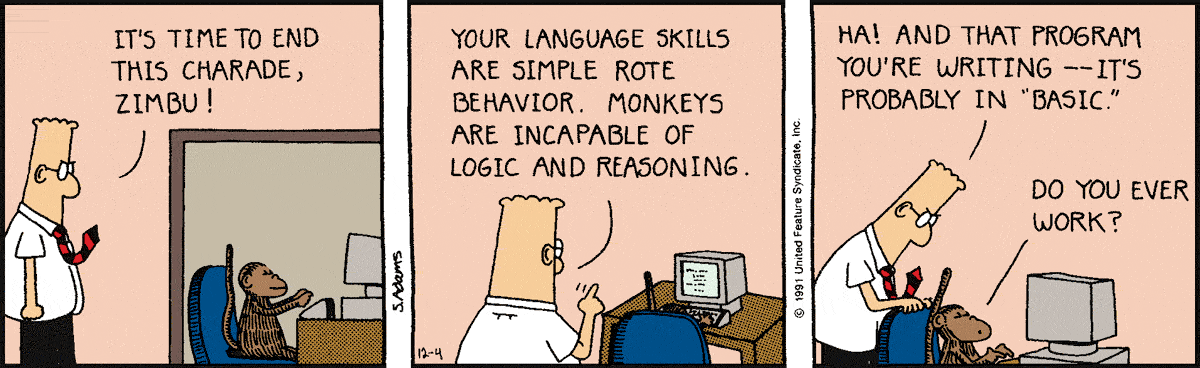
\includegraphics[width=\textwidth]{figs/dilbert-1991-12-04.png}

%% \makequotation{\ldots the teaching of BASIC should be rated as a
%%   criminal offence: it mutilates the mind beyond recovery.}{Edsger
%%   W. Dijkstra, Turing Award winner}

%% \makequotation{I think it's fair to say that more persons in the world know how to
%% write simple programs in BASIC than in any other language. It is true
%% that most of them are probably still unable to vote or buy a drink.  And
%% if FORTRAN is the lingua franca, then certainly it must be true that
%% BASIC is the lingua playpen.}{Thomas E. Kurtz, co-creator of BASIC, in
%%   1981~\cite{hopl}} 

Much has been written over the decades about the democratization of
computers thanks to Moore's Law, but what has been overlooked is that up
until the consumer Internet appeared in around 1995, BASIC was present
at every milestone, and played a pivotal role in empowering generations
of programmers.
Yet BASIC is probably one of the most maligned programming languages
to achieve widespread use.

In \emph{Back to BASIC}~\cite{backtobasic}, the language's co-creators
object that the criticisms leveled at the 
BASIC dialects that proliferated after BASIC became the
\emph{lingua franca} of PCs did not apply to the original language
they had created and to its designated descendants.
This defense seems doubtful, since the original language did include
\T{GO~TO}, which Dijkstra famously railed
against~\cite{goto_considered_harmful}.

In the 2006 Salon article~\cite{why_johnny_cant_code},
science fiction author David Brin laments that for all its flaws, 
despite its small view of the world (or perhaps because of it), BASIC
was sufficiently nonthreatening to introduce an entire generation of
newbies to the joy of programming---exactly the goals of its
creators---whereas today's more expressive languages for higher-powered
platforms may scare beginners away.
Many angry responses to Brin's article pointed out that BASIC
instills habits contrary to modern object-oriented programming practices (true),
that powerful scripting languages like Perl and Python have filled BASIC's
niche (true), and so on.  

In both pieces of writing, the criticisms as well as the responses miss
the point.
Perl and Python are indeed better designed than BASIC, but they are
targeted at professional programmers, not beginners, and they reflect
two decades of thinking and experience focused on a professional
audience, not a student audience.
These languages can be intimidatingly powerful for beginners (though
Python can be suitably simplified by simply not using some of its
advanced
features).\footnote{\href{http://quitebasic.com}{QuiteBASIC.com}, an
in-browser BASIC environment developed in response to Brin's article, is
a good proxy for the ``old school BASIC'' Brin praises.}

The real goal of BASIC was to expose as many non-programmers as possible
to programming---and this it accomplished beyond its creators' wildest
dreams, if not in the precise manner they had envisioned.
With the help of a wide cast of characters who wittingly or unwittingly
played key roles in BASIC's dissemination---Bob Albrecht, David Ahl,
Paul Allen, Dennis Allison, Bill Gates, Chuck Peddle, Ed Roberts,
Li-Chen Wang, Steve Wozniak, and the companies and institutions where
they worked---BASIC introduced an entire generation of programmers to
programming.
If it inculcated ``bad'' habits in us that structured languages tried to
break, it also taught us computational thinking.

It's time the true story of BASIC's influence was told.


\section{UNIVERSAL ACCESS AND COMPUTATIONAL THINKING}

%% \makequotation{Thinking like a computer scientist means more than being able to 
%% program a computer. It requires thinking at multiple levels of
%% abstraction.}{Jeannette M. Wing, \emph{Computational
%%     Thinking}~\cite{wing_computational_thinking}} 

\makequotation{I think everyone should learn how to program a computer,
  because it teaches you how to think.}{Steve Jobs~\cite{steve_jobs_interview}}


For a while in the 80s and 90s, ``computer literacy'' meant familiarity
with productivity tools such as email, Web browsers, word processors,
spreadsheets, and so on.
But within the computer science community, discussions about computer
literacy have always been framed quite differently.
In 1996, MIT computer scientist and educator \w{Seymour Papert} coined
the term \w{computational thinking} to describe the mindset and types of
techniques that characterize a computer scientist's view of
problem-solving.
Ten years later, an
\href{http://www.cs.cmu.edu/afs/cs/usr/wing/www/publications/Wing06.pdf}{influential
op-ed} by Carnegie-Mellon University computer scientist Jeannette Wing
argued for the practical importance of computational thinking and
problem solving~\cite{wing_computational_thinking}.
In 2013, two influential computer scientists, remarking on the demand
for computational thinking in virtually every career path \emph{outside}
of computer science,
stated simply
``Computing is the new
literacy.''~\cite{ieee_computer_special_issue_computing_education}.
%% The ``digital divide'' is no longer about citizens lacking 
%% access to computers, but about citizens lacking \emph{understanding} of how
%% they perform 
%% their tasks and how they augment human intellect.  As Rushkoff says, in
%% this environment we must either ``program or be
%% programmed''~\cite{rushkoff}.

In 1962, Tom Kurtz, a mathematics professor at Dartmouth concerned about
all of these same issues, approached his department chair John Kemeny
with a remarkably farsighted vision: Since computers were clearly going
to be important in everyday life, \emph{all} Dartmouth students should
become computer literate.
This was a radical proposal at a time when computers were so expensive
that they could only be rented, at a monthly cost typically exceeding a
professor's salary, so most universities charged students for actual
computer time used, incentivizing them to minimize actual usage.
Kurtz wanted students to have computer access as easily as they could
borrow library books---just type their student ID number into a
computer and they could start working.
Further, Dartmouth was not an engineering school, but a liberal arts
college where 75\% of the students were nontechnical majors~\cite{goto}.

Like many premier universities, Dartmouth could mitigate the cost of
acquiring computers for education by cultivating good relationships with
computer manufacturers and raising funds from donors and government
grants.
But Kurtz would also need to overcome a technology problem.
``Computer literacy'' meant learning to write simple programs,
but programmers in 1962 had to prepare programs on decks of punched cards,
submit them to a technician,
% TBD picture of punched card
and come back hours or days later to pick up a printout with
the results of their program run.
(It may seem ridiculous today to wait hours or days for the results of a
running a computer program, but given the speeds of 
communication and transportation in 1962, it was normal for
business information to be a few days out of
date~\cite{ceruzzi}.) 
%% If the results were botched because of a simple error in the program,
%% the programmer would re-punch the offending cards, resubmit the job, and
%% again wait hours or days for a result.
%% This method of working, called \w{batch processing}, guaranteed the
%% computer would never be idle as long as there was a long queue of user
%% jobs waiting.
Such \emph{batch processing} favored efficient use of computer time rather
than programmer convenience, an understandable
tradeoff given the high cost of computers.
Kurtz feared that liberal arts students with no
extrinsic career motivation to learn computing would be unwilling
to endure these rituals.
Fortunately, a technical milestone saved the day.
Professor John McCarthy, then at MIT, had been part of a group working
on an experimental technology called
\w{timesharing}~\cite{corbato62timesharing}, in which a computer
switches its attention many times per second among jobs corresponding to
different users.
Because the computer can switch its attention much more quickly than
users can read or type, each user has the illusion that the computer
is waiting only on him or her.

McCarthy easily persuaded Kurtz and Kemeny that such interactive
computer use would be perfect for education because it would allow
students to get
immediate feedback, eliminating the annoying rituals of batch
processing that might discourage beginners.
Although timesharing would turn out to be a revolutionary
technological innovation, 
it wasn't taken seriously in industry at that time since batch
processing provided a more efficient use of the expensive computer's
time.  
In fact, IBM's landmark System/360 line of computers, on which the
company had staked its future in business computing, was rather visibly
rejected by MIT in 1964 because it did not implement hardware-assisted 
address translation (i.e., virtual memory), which MIT considered
essential for supporting timesharing~\cite{ibm360history}.
Dartmouth would
follow MIT's lead, acquiring a less-powerful General Electric computer that
did include dynamic address translation and creating their own timesharing
operating system for it.

\begin{tangent}
Dartmouth's timesharing system was ultimately so successful that it
catapulted GE into a new timesharing business that was profitable for a
few years, and led GE to later offer Dartmouth a brand-new model
computer in exchange for collaboration on re-creating timesharing and
BASIC on it.
\end{tangent}

\smallpicfigure{figs/ASR33.jpg}{fig:ASR33}{The venerable Teletype ASR-33
printing terminal, which integrated a paper tape punch and reader.
Its distinctive uppercase-only font is used in the section headings of
this article.
You can see one in action at https://www.youtu.be/ObgXrIYKQjc---try to
imagine the noise level in a room full of these.}

%% ASR-33 internals in action: https://www.youtube.com/watch?v=11Bcfr8zBvg
%% ASR-33 in action: https://www.youtube.com/watch?v=izC9rIvVnE0

Another challenge was that timesharing would also increase costs:
if many students could use the computer at the same time, each student
would need their own terminal for typing in programs.
Fortunately, although video monitors were still a decade away, 
%% and popular printing terminals
%% were slow and expensive---the
%% Friden Flexowriter printed only 10 characters per second and
%% \href{http://retrotechnology.com/herbs_stuff/flex_behr.html}{cost
%%   \$2500-4000}, or nearly \$20,000 in 2014 dollars.
the Teletype Corporation had recently designed a rugged and
inexpensive ``teleprinter'' for the US~Navy, the Model~ASR-33 (Automatic
Send/Receive terminal).  Teletype made the ASR-33
available to the retail market in 1963 at a price of only \$700 (\$5,200
in 2014)---about a quarter of the price of existing printing
terminals---and sold over
half a million of them before discontinuing the product in 1981.
Dartmouth acquired several ASR-33s to equip the new interactive
timesharing computer lab.


So BASIC was born just when the rapid shift from batch processing to
timesharing began, and as a result
was the first programming language to include a command that made
the program pause and wait for the user to type
something.  Such a concept made no sense in batch processing and was
absent from the high level languages such as FORTRAN and COBOL that had
been developed up to that time.
 


\section{DARTMOUTH, 1964 - KEEP IT SIMPLE}

\makequotation{In cases where there is a choice between simplicity and efficiency,
simplicity is chosen.}{Time Sharing Project Memorandum \#1,
Dartmouth College, November 6, 1963~\cite{hopl}} 

Kemeny initially tried to convince Kurtz to teach students FORTRAN, a
very successful high-level language invented by IBM in 1957 for
scientists and engineers to express mathematical problems.
The key to the FORTRAN system was a special program called a
\emph{compiler} that ingested programs written in the FORTRAN language
and translated them into the much larger number of low-level
computer operations required to carry out the program's tasks.
But Kurtz felt strongly that FORTRAN's notation, which simplified
the compiler while still looking familiar to scientists
and engineers, would drive
nontechnical learners away.

\begin{tangent} 
%% In contrast, BASIC  doesn't require declaring variables in advance, 
%% doesn't distinguish between
%% integers and floating-point numbers (there's a single numeric type,
%% which is roughly double-precision floating-point), and
%% has a Boolean-valued conditional
%% statement with the easy-to-remember syntax \T{IF}~\emph{cond}
%% \T{THEN}~\emph{label}.
The fundamental concepts of compiler construction are well understood
today and routinely taught to computer science 
undergraduates,
but FORTRAN was the pathbreaker and had to wing it. 
The simplest programming-language
parser (the 
\w[History of compiler construction]{LR parser}) was ten years in the
future (it would be invented by computer science legend Donald Knuth),
and parser generators like \T{yacc} certainly didn't exist.
So it's understandable that FORTRAN's language syntax
reflects some concessions to ease of parsing, such as assuming that
variable names beginning with letters I through N always represent
integers (consistent with mathematical notation, 
but seemingly arbitrary to non-mathematicians)
or that the conditional branch statement was originally an arithmetic
condition of the form
\T{IF}~\emph{expression,label1,label2,label3} (easy
to parse,
but much less readable for novices than BASIC's \T{IF}~\emph{condition}
\T{THEN}~\emph{do-something}).

\end{tangent}

Kemeny was persuaded by Kurtz's argument that a new language 
designed specifically for nontechnical beginners was needed.
It would be designed for ease of learning
and ease of use, since only \emph{reasonable} performance was necessary
for the simple programs beginners would write.
Kurtz called the language BASIC, for Beginners' All-purpose Symbolic
Instruction Code.
BASIC  borrowed good ideas from other languages:
for example, like COBOL\footnote{COmmon Business-Oriented Language, designed for creating
business applications such as payroll and inventory.}, every line in a BASIC
program would start with one of the 15 English-like \emph{keywords} in
Figure~\ref{fig:keywords},
making its syntax consistent and easy
to learn.

\tablefigure{figs/keywords.tex}{fig:keywords}{BASIC in one table.  Although some dialects later departed from the
convention that all statements must begin with one of these 15 keywords, the characteristic
was retained and exploited by Woz's Apple Integer BASIC and by Sinclair
ZX80 BASIC~\cite{zx80_basic_techreport}
to check the syntax of each line as it was typed in, rather than when
the program was run.  All
  variables are global; all numbers are floating-point (as in JavaScript); string
  variable names are suffixed with \$.  BASIC's \T{READ} and \T{DATA} statements are based on their
  counterparts in FORTRAN, but whereas FORTRAN's \T{READ} consumes
  values from data cards in the deck, BASIC's \T{READ} consumes values from a
  separate \T{DATA} statement.
}

BASIC also tried to shield beginning users from having to deal with
the operating system's command line, which was as confusing in 1964 as Unix is to
nontechnical learners today.
Much as today's graphical user interface replaced the command line for
most users (you just drag files to folders, without worrying about how
the file storage actually happens), Kurtz added the commands
\T{SAVE} and \T{OLD} to store and later retrieve a copy of the
program you were working on, an operation that otherwise required
an arcane incantation 
like the one in Figure~\ref{fig:jcl_example}.
The inclusion of ``faux OS'' commands persisted in PC BASICs
for operations such as storing programs on cassette tapes.

\codefilefigure{figs/jcl_example.txt}{fig:jcl_example}{%
This code in JCL (the Job Control Language used on IBM
mainframes, analogous to a shell script or 
Makefile today) creates a copy of \T{OLDFILE}
with the name \T{NEWFILE}.}

These concessions to beginners posed challenges for the heroic team of
undergraduates who implemented the first BASIC compiler,
but they did make the language easy to learn.
The original 1964 BASIC manual~\cite[p. 14]{dartmouth_basic_manual}
contains the following instructions for students:
Walk up to an ASR-33 terminal, type \T{HELLO}, enter your student ID
number when prompted, and type the name of the system you want to use
(\T{BASIC}).
That's the entire contents of the section on ``how to use the computer
system'': three double-spaced pages, one of which is a full-page diagram of the ASR-33
keyboard explaining keys such as \T{CTRL} and \T{ESC} to 1964
typists.

% (film: montage of power-on sequences of various home computers)

The use of timesharing rather than batch processing influenced
BASIC's syntax as well.
With programs entered on a line-at-a-time printing terminal
(affordable video display
terminals were years away) rather than supplied on decks of punched
cards, how could learners easily specify the order of program execution
as they typed in program lines?
The ingenious solution was that each line in a BASIC
program would begin with a number, and the program would be
executed in order of ascending line numbers, which didn't have to be
consecutive.  
It didn't matter in what order the lines were entered;
typing \T{LIST} would show
you all or part of your program in line-number order,
and beginners were encouraged to leave gaps in line
numbering (10, 20, 30, etc.) so they could add
more lines later.  (To delete a line, you just entered a line
consisting of the line number only.)

  \begin{tangent}
  The convention of line numbers was retained in virtually all ``street
  BASICs'' long after cursor-addressable CRT terminals were ubiquitous,
  and was finally dropped in Microsoft Visual Basic (although many modern
  BASICs, including VB, still allow them).
  \end{tangent}

BASIC was also the first high-level language to include a keyword
(\T{INPUT}) that means ``stop and wait for
the user to type something,'' a concept that makes no sense in batch
processing. 

Dartmouth's collaboration with General Electric on creating BASIC and
a timesharing OS for their computer would be pivotal in two other
ways.
First, General Electric engineer Chuck Peddle was among the first
non-Dartmouth engineers to be exposed to BASIC, literally the day
after the language was invented~\cite[p.~5]{commodore}.
Fifteen years later, Peddle would design the 6502 microprocessor,
which launched the PC revolution.  Peddle's choice of
BASIC as the language to ``build into'' those first hobbyist computers would turn it
into the most widely-used computer language in the world.
Second, because of the success of timesharing, GE opened a handful of
regional computing centers offering Dartmouth BASIC.
One of these centers, in Seattle, attracted a talented high school
student named Bill Gates~\cite{basic_history_gdm}, who would later launch one of the
world's most successful software companies by creating a
version of BASIC for then-brand-new personal computers.
But while Gates finished high school and entered Harvard University as
an undergraduate, a cultural revolution was brewing that would set
Gates's future company on a collision course with the hippies of
northern California.


\section{PALO ALTO, 1970 - COMPUTING FOR EVERYONE}

%  what did 'universal access' mean in the culture of 1970 CA?

Fast forward to 1970 California, when the first personal computers (Altair,
Mark-8) were becoming available.  Bob Albrecht, a refugee from computer
maker Control
Data, had become uneasy with the industry's emphasis on computers for
corporations rather than people.  He 
started the People's Computer Company in Menlo Park, a nonprofit walk-in
computer center where anyone could walk in and pay per hour to use
terminals connected to a PDP-8 and (later) a remote Hewlett-Packard
mainframe computer on which 
HP had donated time.  People wrote and ran small-business programs, played games
(mostly written in BASIC), and so on.
A frequent visitor was Ted Nelson, an early proponent and visionary of
the idea of linked hypertext.  Like Kurtz, Nelson believed computers
would be important and everyone should learn about them; the rallying
cry of his book \emph{Computer Lib/Dream Machines} was ``You can and
you must understand computers now!''

Albrecht convinced colleague Dennis Allison, an idealistic Stanford
lecturer, to create an \w{open source} ``\w{Tiny BASIC}'' that would run
on the emerging PCs, most with less than 4KB RAM, so that programming
might be accessible to all.  (Albrecht would later help co-author the introductory programming manual
that came with the breakthrough \w{Commodore VIC-20}
computer~\cite{commodore}.) 
Dennis and Bob started the newsletter \emph{Dr. Dobb's Journal of Tiny BASIC
Calisthenics and Orthodontia} (``Dobb'' is a contraction of their names)
as a sister publication to the People's Computer Company newsletter to
publish information about Tiny BASIC.
By overwhelming reader demand, the quirky newsletter was eventually
turned into a full-fledged monthly publication for computer enthusiasts
named simply \w{Dr. Dobb's Journal}, which continued in print
until 2009 and still circulates online.

Palo Alto Tiny BASIC and the TRS-80 Model I

\begin{milestone}{Open source}

\end{milestone}


\section{CAMBRIDGE 1975 - GATES - ALLEN - ALTAIR}

% transition/tech milestone: the microprocessor - 4004, 8008, 8080

\makequotation{%
\emph{Interviewer:}\/ What do you consider your greatest achievement ever in
programming? \\
\emph{Bill Gates:}\/ I'd have to say BASIC for the 8080, because of the effect it's
had, and because of how appropriate it was at the time, and because we
managed to get it so small. It was the original program we wrote when we
decided to start Microsoft.}{1994 interview with Bill Gates~\cite{smithsonian_interview}} 

Gates, a Harvard undergraduate, and his colleague 
Paul Allen, a college dropout working as a programmer for Honeywell
in Boston, had shared an enthusiasm for computing since they were
teenagers growing up together in Seattle.
When the Altair 8800 was announced,
Allen persuaded Gates that personal computers were coming quickly.
Like Bob Albrecht, the pair immediately realized that all those
computer owners would want to write programs, there being no serious third-party
software industry at that time.
But where Albrecht saw a way to extend the ``share alike''
counterculture via open source, Allen and Gates saw a business opportunity.

Gates had
previously written a BASIC interpreter for  a DEC \w{PDP-10}
minicomputer 
as a  high school project.  Gates believed interpreters were better for
learning because of the instant feedback they gave:
``[y]ou could just type
the thing in and immediately see what was
happening.''~\cite{smithsonian_interview} 
And interpreters can be implemented in less memory than compilers,
an important advantage given the paltry 4KB~RAM in the entry-level  Altair.

So Gates and Allen began writing a BASIC interpreter in Intel 8080
assembly language for the
Altair~8800 and the other personal computers they
knew would soon follow.
When Gates remarked during a dinner conversation at Harvard
that he didn't know how to handle floating-point arithmetic in his
BASIC, fellow student Monte Davidoff chimed in with ``I can do that.''
At the time, there was no standard for implementing floating-point in
computer languages, so Davidoff designed his own scheme, probably based
on the techniques used by the DEC~PDP-10 and other DEC minicomputers of
that time.

  \begin{tangent}
  Implementing
  floating-point arithmetic in a rigorous manner was so tough that Intel 
  and other chip vendors eventually convened a technical committee to
  research the problem, under the aegis of the Institute of Electrical and 
  Electronics Engineers (IEEE), a vendor-neutral professional and scholarly
  society. 
  UC~Berkeley professor \w{William Kahan}
  ultimately received the 
  Turing Award for
  leading the effort~\cite{kahan_interview}, whose results were codified as
  the \w[IEEE floating point]{IEEE-754} standard in 1985.
  \end{tangent}

Gates faced new problems in adapting BASIC to PCs.
How could his BASIC interact with the underlying hardware of 
the Altair computer, which had no operating
system?
Fortunately inspiration was near at hand:
In 1971, DEC had had to solve a similar problem 
on the wildly popular PDP-11 computer, successor to the PDP-10 Gates had
programmed in high school.
The PDP-11 had a 
timesharing OS called \w[RSTS/E]{RSTS} (``Resource sharing, time
sharing'') much of which was implemented in BASIC\footnote{This is not as
  ridiculous as it sounds given that BASIC was compiled.  After all,
   Unix is implemented largely in C.}, so DEC had added
three new commands to allow interaction between BASIC programs and the
hardware: \T{SYS} to make a system call to a
known logical address from a BASIC program, and
\T{PEEK} and \T{POKE} to query and set the contents of individual memory
bytes (like C \texttt{unsigned char~*}
pointers)~\cite[pp.~204--205]{ceruzzi}.
Gates put all three into Altair BASIC~\cite{smithsonian_interview},
with \T{SYS} renamed to \T{USR} for User Service Routine; all three
survived in virtually every PC adaptation of BASIC.

In an impressive feat of programming, Gates squeezed a 
feature-laden and high-performing BASIC interpreter into the Altair's
paltry 4K~RAM.
Gates later recounted that the extensive tuning gave the authors
confidence of the superiority of their work~\cite{programmers_at_work}.
The feat is even more impressive considering that none of the team had
access to an actual 8080 or Altair computer: the whole project was done
using an 8080 emulator Gates had written to run on Harvard's student
computer system, and it wasn't until they loaded the code into actual
Altair hardware during their first demo at the MITS offices  in Albuquerque
that they knew conclusively that it worked.
The high-stakes demo was a success, and Allen quickly set up shop in
Albuquerque as Micro-Soft [sic].
Microsoft BASIC was not only the product that launched a juggernaut
company, it was also Bill Gates's baby.

\begin{tangent}
Not only had the BASIC interpreter never been tested on real hardware:
during the flight to Albuquerque, Allen realized they hadn't thought
about how to load the interpreter code into the Altair to begin with.
The Altair had no BIOS or boot ROM, so while on the plane, Allen wrote a
simple ``boot loader'' program that, when entered manually into the
Altair by toggling switches to enter one assembly-language instruction
at a time, would be able to read the rest of the interpreter code from
paper tape.  Just-in-time programming, indeed!
\end{tangent}

But Gates and Allen now faced a cultural obstacle in trying to sell their
BASIC.
In early days of computing, the excitement and innovation was around hardware.
Software was an afterthought---something you learned to do in order to
use your nifty new hardware, or if you were a computer company,
something you gave away for free to stimulate hardware sales.
The ``share-alike'' mindset promulgated by Albrecht and his California
colleagues wasn't helping:
in Palo Alto's Homebrew
Computer Club, where a young Steve Wozniak would
eventually demonstrate the Apple~I, it
was considered socially acceptable to
make copies of software  to give your friends---it even enhanced
your standing as a club member if you provided something useful.
The idea of a separate software industry, in which
people paying for software could be a major economic driver of the PC era,
was simply not in most people's sights.  

But Bill Gates was not most people: in 1976 he laid out just this vision,
perhaps somewhat abrasively, in a now-infamous ``open letter to computer
hobbyists'' published in the 
MITS newsletter that all Altair owners received.
In pointed language, Gates railed against the ``software pirates'' who
circulated paper tape copies of Micro-Soft BASIC, complaining that they
were stealing 
his work and making a third-party software industry financially
infeasible.
The culture clash could not have been greater.
Notwithstanding the hue and cry generated by the letter, Gates
quickly figured out that a better solution was to license BASIC directly
to computer manufacturers, who would burn it into the ROM of each
computer sold, much as a BIOS is today.
(This pattern would be repeated later with Windows, which would be
licensed by computer manufacturers to preinstall on new PC hard drives,
rather than purchased separately by the end user.)

So Bill Gates successfully got BASIC running on the first personal computer, but that computer was only
accessible to hobbyists who could solder and who would tolerate using
something that looked more like a piece of lab equipment.  The Altair had no way
to accept or display text, let alone graphics, without adding additional
hardware. 
Gates knew that a ``ready-to-run'' computer was inevitable, but he was a
software designer.  Fortunately, a hardware designer who had also been
bitten by the BASIC bug was taking up the challenge---not in northern
California, nor even in Boston, but in the unlikely town of Valley Forge,
Pennsylvania, where General George Washington had pulled his army
through the bitter winter of the American Revolution nearly 200 years before.




\section{VALLEY FORGE, 1975 - THE 6502}

\begin{milestone}{The 6502}
% milestone: the 6502.  made truly inexpensive home computers possible
% (with all due respect to sinclair)

\end{milestone}

Chuck Peddle,  who had been working at General Electric when BASIC was
born at Dartmouth, had since moved on to chip maker Motorola, whose 6800
processor chip had been introduced to compete with the Intel 4004 and
8008, the earliest microprocessors that were originally developed for
electronic calculators.  The 6800 sold successfully for \$300, but
Peddle  believed that with a few tweaks they could
produce a competitive product that could sell for a fraction of the
price: a \$20 price
point would ``put
microprocessors everywhere''~\cite[p. 31]{commodore} and make it possible for
manufacturers of all kinds of appliances and equipment to become
Motorola customers.

Unable to get Motorola interested, Peddle and a few of his close
colleagues left to start their own company, MOS Technology\footnote{MOS stands for metal oxide
semiconductor, a phrase that describes the breakthrough technology that
made integrated circuits (computer chips) possible.}.

Peddle's strength was in the logical design of the chip and in his years
of experience with how these chips would be used in ``real world''
programs and systems.
By selectively omitting some rarely-used 6800 features and enhancing
others, Peddle 
created a simple and flexible design that required only 4300
transistors.
(By comparison, complex Intel microprocessors in 2012 use over 1
billion transistors!)
The simple design made the chip smaller, an important advantage since
chip manufacturing costs were dominated by the ceramic or plastic
package (picture) the chip was mounted in.
The simple design was laid out and hand-drawn by hand by Bill Mensch,
hand-simulated by the other engineers, and hand-tested on a jury-rigged
chip testing apparatus, since the young company could not afford the
fancy automation used by their competitors.
Meanwhile, Peddle's colleague John Paivinen, an expert in the chemical
and physical manufacturing processes used to produce the chips, had
invented a technology\footnote{Contactless mask liners.} that allowed
the ``master'' from which chips are ``stamped'' to last indefinitely,
rather than wearing out bit by bit as more chips are produced.
With these advantages and careful tuning of the manufacturing process,
typically 70\% of the 6502 chips coming off MOS Technology's assembly
line worked correctly, compared to 30\% yields for competitors.

The result is that MOS Technology could manufacture the chip for \$12
and sell it for \$20 in quantities of one.  The 6502 had been designed
to compete against the simple Intel 4004 and 8008, but as it turned out,
its design and performance made it competitive with the Intel 8080,
which sold for \$360 in small quantities and \$75 to Altair 
in large quantities~\cite[p. 228]{ceruzzi},
and the \$360 Motorola 6800.  The trade paper \emph{Electronic
  Engineering Times} was skeptical that the company could provide good
technical support at such a low price, but a review in the influential
new magazine \emph{Byte}~\cite{byte75:6502} put the 6502 on the radars
of many hobbyists, including Steve Wozniak, who waited in line  to buy
one at the Wescon trade show where it was introduced,
thinking he might be able to use it in the hobbyist computer he was
designing for the Homebrew Computer Club meeting in Palo Alto.  



\begin{geeknote}
Peddle cannily made the 6502 pin-compatible and largely
assembly-code-compatible (but 
binary-incompatible) with the 6800 to take advantage of 
6800 hobbyist kits and existing motherboards, but a lawsuit from
Motorola soon put a stop to that.
\end{geeknote}


(In a similar vein, Steve Wozniak would hand-assemble the Integer BASIC that
shipped with the original Apple ][ (and which bears a striking resemblance to
 HP BASIC) and Bill Gates hand-optimized his 8080 BASIC, which ran on
 native hardware for the first time during its critical demo at MITS.)

%% In 1974, HP introduced the HP-65 programmable calculator, Intel
%% announced the 8080, and (in December) \emph{Popular Electronics} had the
%% Altair 8800 on the cover.  


    \begin{geeknote}
The 6502 reflected good engineering taste in what to leave out.
Compared to the 6800, the 6502 lacks the second accumulator, the
tristate drivers for the address bus (so you can't do DMA, which was seen as
unnecessary for small systems~\cite{byte75:6502}), 
and the 6800's 16-bit index register.  In exchange, the 6502 provides a pair
of 8-bit index registers that enables an additional kind of
indirect addressing with a true index register offset.
This design decision, based on designer Chuck Peddle's experience with real
code and his knowledge of the PDP-11 instruction set, 
reduces instruction count and execution time by up to a
factor of 2 over the 6800 for referencing arrays using random
offsets and for operations that
maintain pointers into two arrays.
As a result, the 6502
beat almost all its competitors on  the AH Systems benchmarks of
the day~\cite{edn75:6502}, despite selling for a fraction of the price.

Since RAM could be accessed in one
clock cycle (the 6502 ran at
1~MHz) , RAM was used as overflow registers instead of devoting valuable die
space to registers.  The ``zero
page'' (bytes 0x0000 to 0x00ff in the 6502's 16-bit address space) had
special load and store instructions that were one byte shorter to fetch and
decode, since the high-order address byte was zero.
The 6502 was the first pipelined
microprocessor, giving it a higher instructions-per-clock 
rate than comparable processors and making
common instructions such as relative
branch and subroutine calls 1 to 3 cycles faster than
on comparable microprocessors.  

Later, the derivative 6507 would
remove some other features and limit
physical memory to a 14-bit address space.  These changes allowed it to
use a 28-pin 
plastic package vs. 40-pin ceramic package and to be sold for \$5,
making it the chip that was chosen for the Atari 2600.
    \end{geeknote}


\section{STREET BASIC BECOMES A MUST-HAVE FEATURE}

\makequotation{I think it's fair to say that more persons in the world know how to
write simple programs in BASIC than in any other language. It is true
that most of them are probably still unable to vote or buy a drink.  
%% And
%% if FORTRAN is the lingua franca, then certainly it must be true that
%% BASIC is the lingua playpen.
}{Thomas E. Kurtz, co-creator of BASIC, in
  1981~\cite{hopl}} 

While the term ``open source'' hadn't been invented in 1964, and BASIC's
original source code itself was not ``open'' as we use that term today, its
inventors made clear that anyone was free to \emph{implement} the language
without a license from Dartmouth.
Perhaps unfortunately, this permissiveness also meant that there was
no standard set of requirements that any particular version of BASIC
had to meet in order to call itself BASIC.


\begin{tangent}{}
In contrast, modern languages are often more tightly protected.
For example, Java implementations must pass an Oracle ``compatibility
suite'' whose licensing terms impose intellectual property constraints
that restrict how you may redistribute your
implementation~\cite{apache-java-letter,apache-resigns-jcp}.
 ``Minimal BASIC'' was standardized by the American
National Standards Institute in 1978, but by that time, many variants
of the language had already proliferated and the standard was largely ignored.
\end{tangent}

Nonetheless, precisely because BASIC was unencumbered and easy to learn, it quickly became
influential not only in colleges and universities, but among PC
makers.
Indeed, as Chuck Peddle had foreseen, PC vendors soon realized that a
computer \emph{without} BASIC built in was a competitive liability.
Sphere Computer and Processor Technology boasted low-cost computers
whose BASIC was vaporware at the time of introduction and
underperformed when finally released~\cite[p. 114, 134]{veit}; both
companies quickly went under.
When Steve Jobs demonstrated the prototype Apple~I at a
conference\footnote{Actually a dinner meeting of the New York chapter
of the Association for Computing Machinery, the first and largest
professional society for computing professionals.} in
1976, the technical attendees were astonished at the hardware, but
dealers' reactions amounted to ``call us when BASIC is available.''
Jobs said Woz was ``working hard'' on BASIC for the follow-on
Apple~II~\cite[pp. 92ff]{veit}, which was true---on August 26, 1976,
two nights before the first national computer show in Atlantic City,
not far from New York, Woz was using the TV in  his hotel room as a
monitor,  finishing work on Apple
``Integer BASIC'' in time to demonstrate it at the show.

\begin{tangent}
Unlike Gates, Woz knew little about interpreters or compilers, he
couldn't afford an assembler program, and his knowledge of BASIC was
based on a few hours at a high school terminal and his job at
Hewlett-Packard, whose mainframe computers had BASIC on them.
Woz was primarily interested in writing games, so his Apple BASIC
included commands to draw color graphics and read the position of a
joystick, but no floating-point arithmetic or file I/O.
\end{tangent}

\smallpicfigure{figs/breakout.jpg}{fig:breakout}{The \emph{Breakout}
  game implemented in Apple Integer BASIC.  According to Woz
  himself~\cite{woz-basic}, being able to easily create games like this one,
  which he had designed for Atari a few years before, was his
  main goal for Apple BASIC.}

The trend was clear: users expected to turn on their PCs and start
programming in BASIC, courtesy of a ROM-based interpreter.
And Micro-Soft was perfectly positioned to take advantage of this
trend.
Unlike Gates the software wizard, Woz was really a hardware specialist, so
his Apple BASIC was inferior to Micro-Soft's.
When investor Mike Markkula joined Apple in 1977
as the new CEO, he quickly negotiated a deal with Gates to port
Micro-Soft BASIC to the Apple~II, paying double what Commodore had
paid~\cite[p. 114]{commodore}.
That same year, Radio Shack made a deal to provide Micro-Soft
BASIC as an upgrade for the TRS-80 Model~I, which shipped with 
the free Palo Alto Tiny BASIC,
again doubling the price that Apple had paid.
Micro-Soft BASIC was now the dominant computer language on the first
three major PCs---the Commodore PET, TRS-80 Model~I, and Apple~II, all
released in 1977.

%% \tablefigure{figs/basics.tex}{fig:basics}{The first crop of ``ready-to-run'' PCs
%%     all featured BASIC in ROM.  Woz's Integer BASIC was written from
%%     scratch; TRS-80 Level~I BASIC was based on Palo Alto Tiny BASIC; the
%%     rest are ports of Microsoft BASIC.}

Although cassettes were widely used by hobbyists as a way to store
programs inexpensively, and floppy disk drives were slowly beginning
to appear, cassette and disk formats were incompatible across
different computer systems.
Cassettes or disks created for a TRS-80 wouldn't work on an Apple or
Commodore, just as today's PC programs don't work on Macs.
So hobbyists had to laboriously type in programs from printed listings
in hobbyist magazines.
Those programs were usually written in Micro-Soft BASIC
(by then the \emph{de~facto} standard),  but as new computers entered
the market and introduced
innovative hardware features such as
graphics and sound, each manufacturer modified their version of 
Micro-Soft BASIC to take advantage of their computers' newest features.
In time, over 60 different PC models implemented BASIC in ROM alone,
not counting later disk implementations such as GWBASIC for MS-DOS.
Like species that gradually become distinct and unable to mate, these
different ``dialects'' of BASIC soon diverged enough that all but the
simplest BASIC programs became vendor-specific, increasing the market
for hobbyist magazines focused on one particular type of computer.

Kemeny and Kurtz, BASIC's original creators, were dismayed at this
proliferation of incompatible dialects and the addition of
\emph{ad~hoc} features that (in their opinion) were often in poor
technical taste and contrary to the original spirit and goals of the
language.
They began using the derogatory term ``street BASIC'' to distinguish
these incompatible mass-market dialects from the original language
they had been curating and using at Dartmouth.
But as university educators, they may have been even more dismayed
that the ``killer app'' for BASIC turned out to be not formal
computing education as they had intended, but\ldots{}games.





\section{INFLUENCE AND LEGACY}

\makequotation{Whether we're still programming in it or not, the spirit
  of BASIC lives on in all of us.}{Jeff Atwood, founder of
  StackExchange and author of Coding Horror blog~\cite{codinghorror_basic}}

With no economical mass storage (floppy disks) coming until 1980, and no
consumer-facing Internet until the 1990s, BASIC programs were
distributed by a far more prosaic medium: you had to type in the source
code from a printed listing.  Students traded source code listings, 
magazines published listings contributed by readers, and in 1972, David
Ahl, then working in the education department of Digital Equipment
Corporation, published a whole book of them---\emph{BASIC Computer
  Games}~\cite{basic_computer_games}. 

Ahl's book had a backstory too.
The mother of all ``type-in'' BASIC games traces its origins to
1971, when Mike Mayfield and some high school friends ``borrowed'' time
on an SDS Sigma~7 computer at UC~Irvine to write a game inspired by the
original \emph{Star Trek} TV series.  \emph{Star Trek} had just ended its 3-season run and
was very popular among computer hobbyists.
In the game, the player commands the USS~Enterprise and moves it around
a grid seeking and destroying Klingon warships.  The grid was rendered
as a set of ASCII text characters, and was redrawn after each turn, so
the game could be played on both printing terminals like the ASR-33 and
the CRT displays that were around the corner.

Mayfield later ported the game to Hewlett-Packard BASIC in exchange for
some time on an HP-2000C timesharing computer at a local HP sales
office.
The HP version was discovered by David Ahl, who (in the share-alike mentality of the day)
immediately ported it to DEC's dialect of BASIC and shared it freely via the DEC
Education Newsletter, encouraging readers to submit their own games.

In 1978 Ahl launched \emph{Creative Computing}, one of the first
magazines focused on emerging microcomputers and featuring lots of
so-called ``type-in programs.''
Ahl ported his original collection of games
to Microsoft BASIC, which had emerged as the
\emph{de~facto} standard for microcomputers, and published the
resulting collection as \emph{BASIC Computer
Games}~\cite{basic_computer_games}.
The book became a staple in high school computer labs and hobbyists'
homes, and was the first computer book to sell over a million copies.

Younger readers may be surprised to learn how many 
surprisingly sophisticated games relied on line-at-a-time text output,
the only output medium guaranteed to be available in all BASIC dialects.
For example, Scott Adams wrote his first interactive text adventure game
in BASIC, and started
the first software company devoted exclusively to game publishing,
Adventure International.\footnote{The earliest interactive text adventure (you type
``Go North''; the computer types back something like ``You are next to a
running stream'') had been
\href{https://armandofox.blogspot.com/2007/08/the-original-original-adventure.html}{written by Will Crowther in FORTRAN.}}
Adams even published a complete game called \emph{Pirate's Adventure} as
a type-in program in a special issue of BYTE devoted to adventure
games~\cite{byte80:adventure}; the article helpfully notes which parts
of the BASIC program would have to be changed to run on other
Microsoft-derived BASIC dialects.

Games were crucial to the success of BASIC on PCs.
Later versions of Star Trek displayed ships as graphic icons rather than
letters and symbols on a text grid.
Scott Adams enhanced his adventures' visual appeal with colorful---albeit
static---images.
\emph{Oregon Trail}, a turn-based simulation based on the US westward
migration and originally written in 1971 by US~history TA Don Rawitsch and colleagues,
received graphic enhancements and became
a bestseller on the Apple~II and other computers;
the millions of
North American elementary school students who played the game in school
in the 1980s--1990s
may be unaware that it was originally text-only.
Strategy game publisher
Automated Simulations published two turn-based simulation games about
space colonization,
% high-quality ``space opera'' games,
\emph{Starfleet Orion} and \emph{Invasion Orion}, that were not only
written in BASIC but could be modified by sophisticated users to
customize the gameplay: since BASIC programs were interpreted, the
companies had no choice but to provide the source code.

\w{Odyssey: The Compleat Apventure} [sic] was a 1980 turn-based adventure game
written in Apple II Integer BASIC
that made extensive (for its time) use of
graphics, using the Apple's ``high resolution'' mode ($280\times 192$, 6 colors)
to display overall maps showing the player's
avatar and major landscape/seascape features, and its
``low resolution'' mode ($40\times 40$, 15
colors) mode to display cave and dungeon interiors in some phases of game play.
Figure~\ref{fig:odyssey} shows some screen shots from the game.

\picfigure{figs/odyssey.png}{fig:odyssey}{Four screenshots from \emph{Odyssey: The Compleat
    Apventure}, written in Wozniak's original Integer BASIC.  Each ``phase'' of the game was
  a completely separate program, loaded \w[Overlay (programming)]{overlay}-style.}

Meanwhile, Commodore, the company under whose umbrella MOS Technology
had produced the wildly popular 6502 microprocessor, had been working on
an advanced video game chip they hoped to sell to home game console manufacturers
such as Atari.
When Commodore was unable to find any customers for the chip, two young
Commodore engineers, Bob Yannes and Al Charpentier, decided instead to
develop an inexpensive computer around it.
The VIC-20 had entry-level hardware but very impressive graphics
compared to its competitors, and at just \$300, it dropped the price
of an entry-level PC by more than half.
Bob Albrecht brought his informal and folksy writing style to the
introductory programming manual that came with the breakthrough
computer~\cite{commodore}.
Not only did the VIC-20 outsell all other computers when introduced in
1982 (over 1 million units), it also stimulated the sales of the first
under-\$100 modem, which came bundled with free trials of various dialup
services including CompuServe and in 1982 accounted for the largest
traffic on that network.
The first bulletin board systems (BBSes)---analogous to dialup
newsgroup servers in the Unix world---were written in BASIC.
A little over a year later, Commodore engineers outdid themselves with
the Commodore~64, the best-selling personal computer of all time (over
10 million sold), featuring spectacular graphics and sound and 64KiB
of RAM for an unheard-of \$595.

\begin{tangent}
Hard-driving Commodore chairman Tramiel may have been the last person to
outsmart Bill Gates.
Tramiel claimed that the wording of the original ``flat fee'' paid to
Microsoft for porting BASIC to the PET allowed Commodore to package
BASIC with every \emph{computer} sold, not just every \emph{PET} sold,
as long as no substantive changes (``derivative works'') were made.
Of course, this meant Commodore couldn't legally modify BASIC to allow
access to the advanced graphics and sound capabilities in the VIC-20 or
Commodore~64, so programmers had to learn bits of 6502 assembly language
to do anything more than rudimentary graphics.
But it allowed Commodore to sell over 1~million VIC-20s and over
10~million Commodore~64s without further payments to Microsoft.
This infuriated Bill Gates, and resulted in an arguably crippled BASIC
unable to exploit these computers' advanced graphics and sound.
But it did allow VIC-20 and Commodore~64 buyers to run many BASIC
programs that had been written for the PET, especially educational
software, making the computers an easy sell into both homes and
schools~\cite[p. 414]{commodore}.
\end{tangent}


BASIC's role in the 1980s is analogous to JavaScript's role in the
1990s: its performance and relative isolation from the hardware
limited
the kinds of programs you could write, but those programs could reach a
huge audience.
But as falling hardware prices enabled PCs to add unique but
idiosyncratic hardware features such as graphics and sound, BASIC
programs that relied on
platform-specific features weren't portable, so the potential audience
for a given BASIC program soon narrowed to the audience for that
platform.  Programs for popular computers such as the Apple II,
Commodore VIC-20, and Commodore 64 still found a wide audience;
less-popular computers such as the TI-99/4A, Atari 400, and others soon
saw their ``shareware'' base contract.

BASIC also provided a new avenue of empowerment for young programmers.
Game designer Richard Garriott started writing games in BASIC at the age
of thirteen, and created his first game offered for sale,
\emph{Akalabeth,} when he was just eighteen.
While that game was perhaps primitive compared to some commercial
competitors written in faster assembly language, it was the first game
to provide a 3D first-person perspective view of the dungeon maze,
albeit a crude one~\cite{akalabeth}.
Garriott went on to become one of the most successful (and
wealthiest) computer game designers in the world; the first version of
his very successful \emph{Ultima} was also written in BASIC.
In principle, any parent could now buy a computer for their child and
sign a distribution agreement to allow the young prodigy's work to
find its market.

As of this writing (2016), cloud-based IDEs such as Codenvy and Cloud9
have come into their own: anyone can fire up a Web browser and
immediately start programming.
For all the criticism of ``street BASIC,'' its user experience was quite
close to this ``programmer appliance'' view, as BASIC's creators
originally intended: when PC users turned on their computers, the first
thing they'd see was a BASIC interpreter prompt, allowing them to jump
right in and start programming.
And program they did: the first PC games and the first PC
telecommunications programs were written in BASIC, magazines published
program listings in it, and one of the world's largest and most
successful software companies got its start with well-crafted BASIC
interpreters.
According to Wikipedia, there are today over 450 extant and extinct
dialects of BASIC.
Some would call that victory.


\section{ARCHAEOLOGY}

\B{BASIC Interpreters, Compilers, and Emulators.}

QuiteBASIC is my personal favorite for meeting the goal of a simple
BASIC that is beginner-friendly.  That said,
Microsoft's DevLabs 
released \href{http://smallbasic.com}{Microsoft Small Basic} in 2008 as a
Technology Preview plug-in to Visual Studio.
The idea is well-intentioned, although hardly small---Small Basic
requires Windows XP or later, meaning a 500
MHz x86 processor, several gigabytes of disk space, and at least 256
megabytes of RAM.
Also, because of Small Basic's explicitly
object-oriented syntax,  a novice must either understand why she
must say \C{TextWindow.WriteLine("Hello world")} to display text on the
screen or accept the arbitrariness of that syntax---one of the very problems
BASIC's creators set out to eliminate.  

A more authentic route for the historically-minded is to use emulators.
You can try a lot of the software yourself, and explore
its source code, thanks to the many great emulators available and the
collection of emulator-compatible disk images floating around the Internet.

\begin{itemize}

\item \href{http://quitebasic.com}{Quite BASIC} is a free in-browser BASIC
  interpreter that is probably closest in spirit to what David Brin
  lamented missing in his Salon article.  It has a graphics canvas
  allowing programs to do simple graphics.

\item \href{http://virtualii.com}{Virtual-][} is an extraordinarily
  faithful Apple II emulator, right down to the sound effects of
  whirring disk drives and dot matrix printing.

\item \href{http://web.archive.org/web/20011211231432/http://www.rjh.org.uk/altair/4k/em/altem.htm}{Altair emulator with BASIC} (Java applet emulator; doesn't run in Safari,
maybe needs earlier JRE?)

\end{itemize}


% computer history museum

\B{Old source code.}
There is a long saga about trying to get access to the original
Microsoft BASIC source code---the 8080 Altair BASIC authored by Bill
Gates, Paul Allen and Monte Davidoff that launched the PC revolution.
The true urtext is still elusive, believed to be locked in Bill Gates's
personal safe.
The Pusey Library at Harvard University has a copy (which you may
inspect but not photograph\ldots{}WTF?) annotated with version number
1.1.
You can read more about this archaeological quest at
\href{http://www.theregister.co.uk/2001/05/13/raiders_of_the_lost_altair/}{Raiders
of the Lost Altair BASIC Source Code}, The Register, May 13, 2001,
which tells the overall story.
\href{http://www.interact-sw.co.uk/altair/other\%20versions/ian.htm}{Quest
for the Holy Source: Ian's Trip to Harvard} tells about Ian
Griffiths's visit to the Pusey Library at Harvard to view version
1.1.
He reports that the library's copy includes a transmittal letter from
Harry Lewis, Dean of Harvard College and a professor of Computer
Science there, who reportedly found this copy of the source code behind
a cabinet in an old CS office.
The letter reports that other computer scientists, including Donald
Knuth, have made ``pilgrimages'' to Harvard to see this copy.

\href{http://www.drdobbs.com/back-to-the-future/184404733}{Bill's
  Lost Code} (a section of the Back to the Future column in this online
issue of Dr. Dobbs' Journal) observes that based on reading this source
code, Gates was indeed a craftsman and hacker, pulling nifty tricks such
as jumping into the middle of an instruction (because a multi-byte
opcode had a different interpretation if you started reading at the 2nd
or 3rd byte) to squeeze a BASIC interpreter into just 4KiB of ROM.

Reuben Harris, a London programmer, has created an
\href{http://web.archive.org/web/20011211233332/www.rjh.org.uk/altair/4k/index2.html}{annotated
disassembly of the actual Altair 4K BASIC} that you can visit thanks to the
Wayback Machine.


\section{ATTRIBUTIONS}

\begin{itemize}
\item ASR-33 image source:
  \href{http://en.wikipedia.org/wiki/File:Teletype_with_papertape_punch_and_reader.jpg}{Wikimedia
    Commons}, license: Creative Commons Attribution-ShareAlike 3.0
  Unported license, author: AlisonW.
\item 
\end{itemize}

\bibliographystyle{plain}
\bibliography{basic}

\end{document}
